\section{Appendix}

\begin{frame}
    \begin{center}
        \LARGE Appendix
    \end{center}
\end{frame}



\subsection{Reservoir Computer の中のダイナミクスについて}
\begin{frame}{Reservoir Computer の構造}
    \begin{columns}[T] % [T] は列を上部で揃えるオプション
  
        \begin{column}{.5\textwidth}
            Reservoir Computer の学習の計量さについて\cite{Bollt}に倣って確認する.
            ここでは 教師データのある学習期間のみを考える.
            \begin{itemize}
                \item $\left\{\mathbf{x}_i\right\}_{i=1}^N \subset \mathbb{R}^{d_x}$: input data.
                \item $\mathbf{r}_i \in \mathbb{R}^{d_r}$: hidden variable. $d_r>d_x$. \begin{itemize}
                    \item $\mathbf{u}_i=\mathbf{W}^{i n} \mathbf{x}_i$. $\mathbf{W}^{i n}$ はランダムに選ばれた 重み付きの $d_r \times d_x$ 行列. 
                    \item $\mathbf{r}_{i+1}=(1-\alpha) \mathbf{r}_i+\alpha q\left(\mathbf{A r}_i+\mathbf{u}_i+\mathbf{b}\right)$. 
                    
                    $\mathbf{A}:$ ランダムに選ばれた 重み付きの $d_r \times d_r$ 行列.$\alpha:$ leaking rate (後述). $\mathbf{b}:$ offset for activation, $0$ とする.
                    
                    $q:$ activation funciton. $\tanh(\cdot)$ など.
                \end{itemize}
                \item $\mathbf{y}_{i+1}=\mathbf{W}^{\text {out }} \mathbf{r}_{i+1}$: output data.\begin{itemize}
                    \item $\mathbf{W}^{\text {out }}:$ 重み付きの $d_x \times d_r$ 行列. データに対して学習される.
                \end{itemize}
            \end{itemize}
        \end{column}
        \begin{column}{.5\textwidth}
            \begin{figure}
                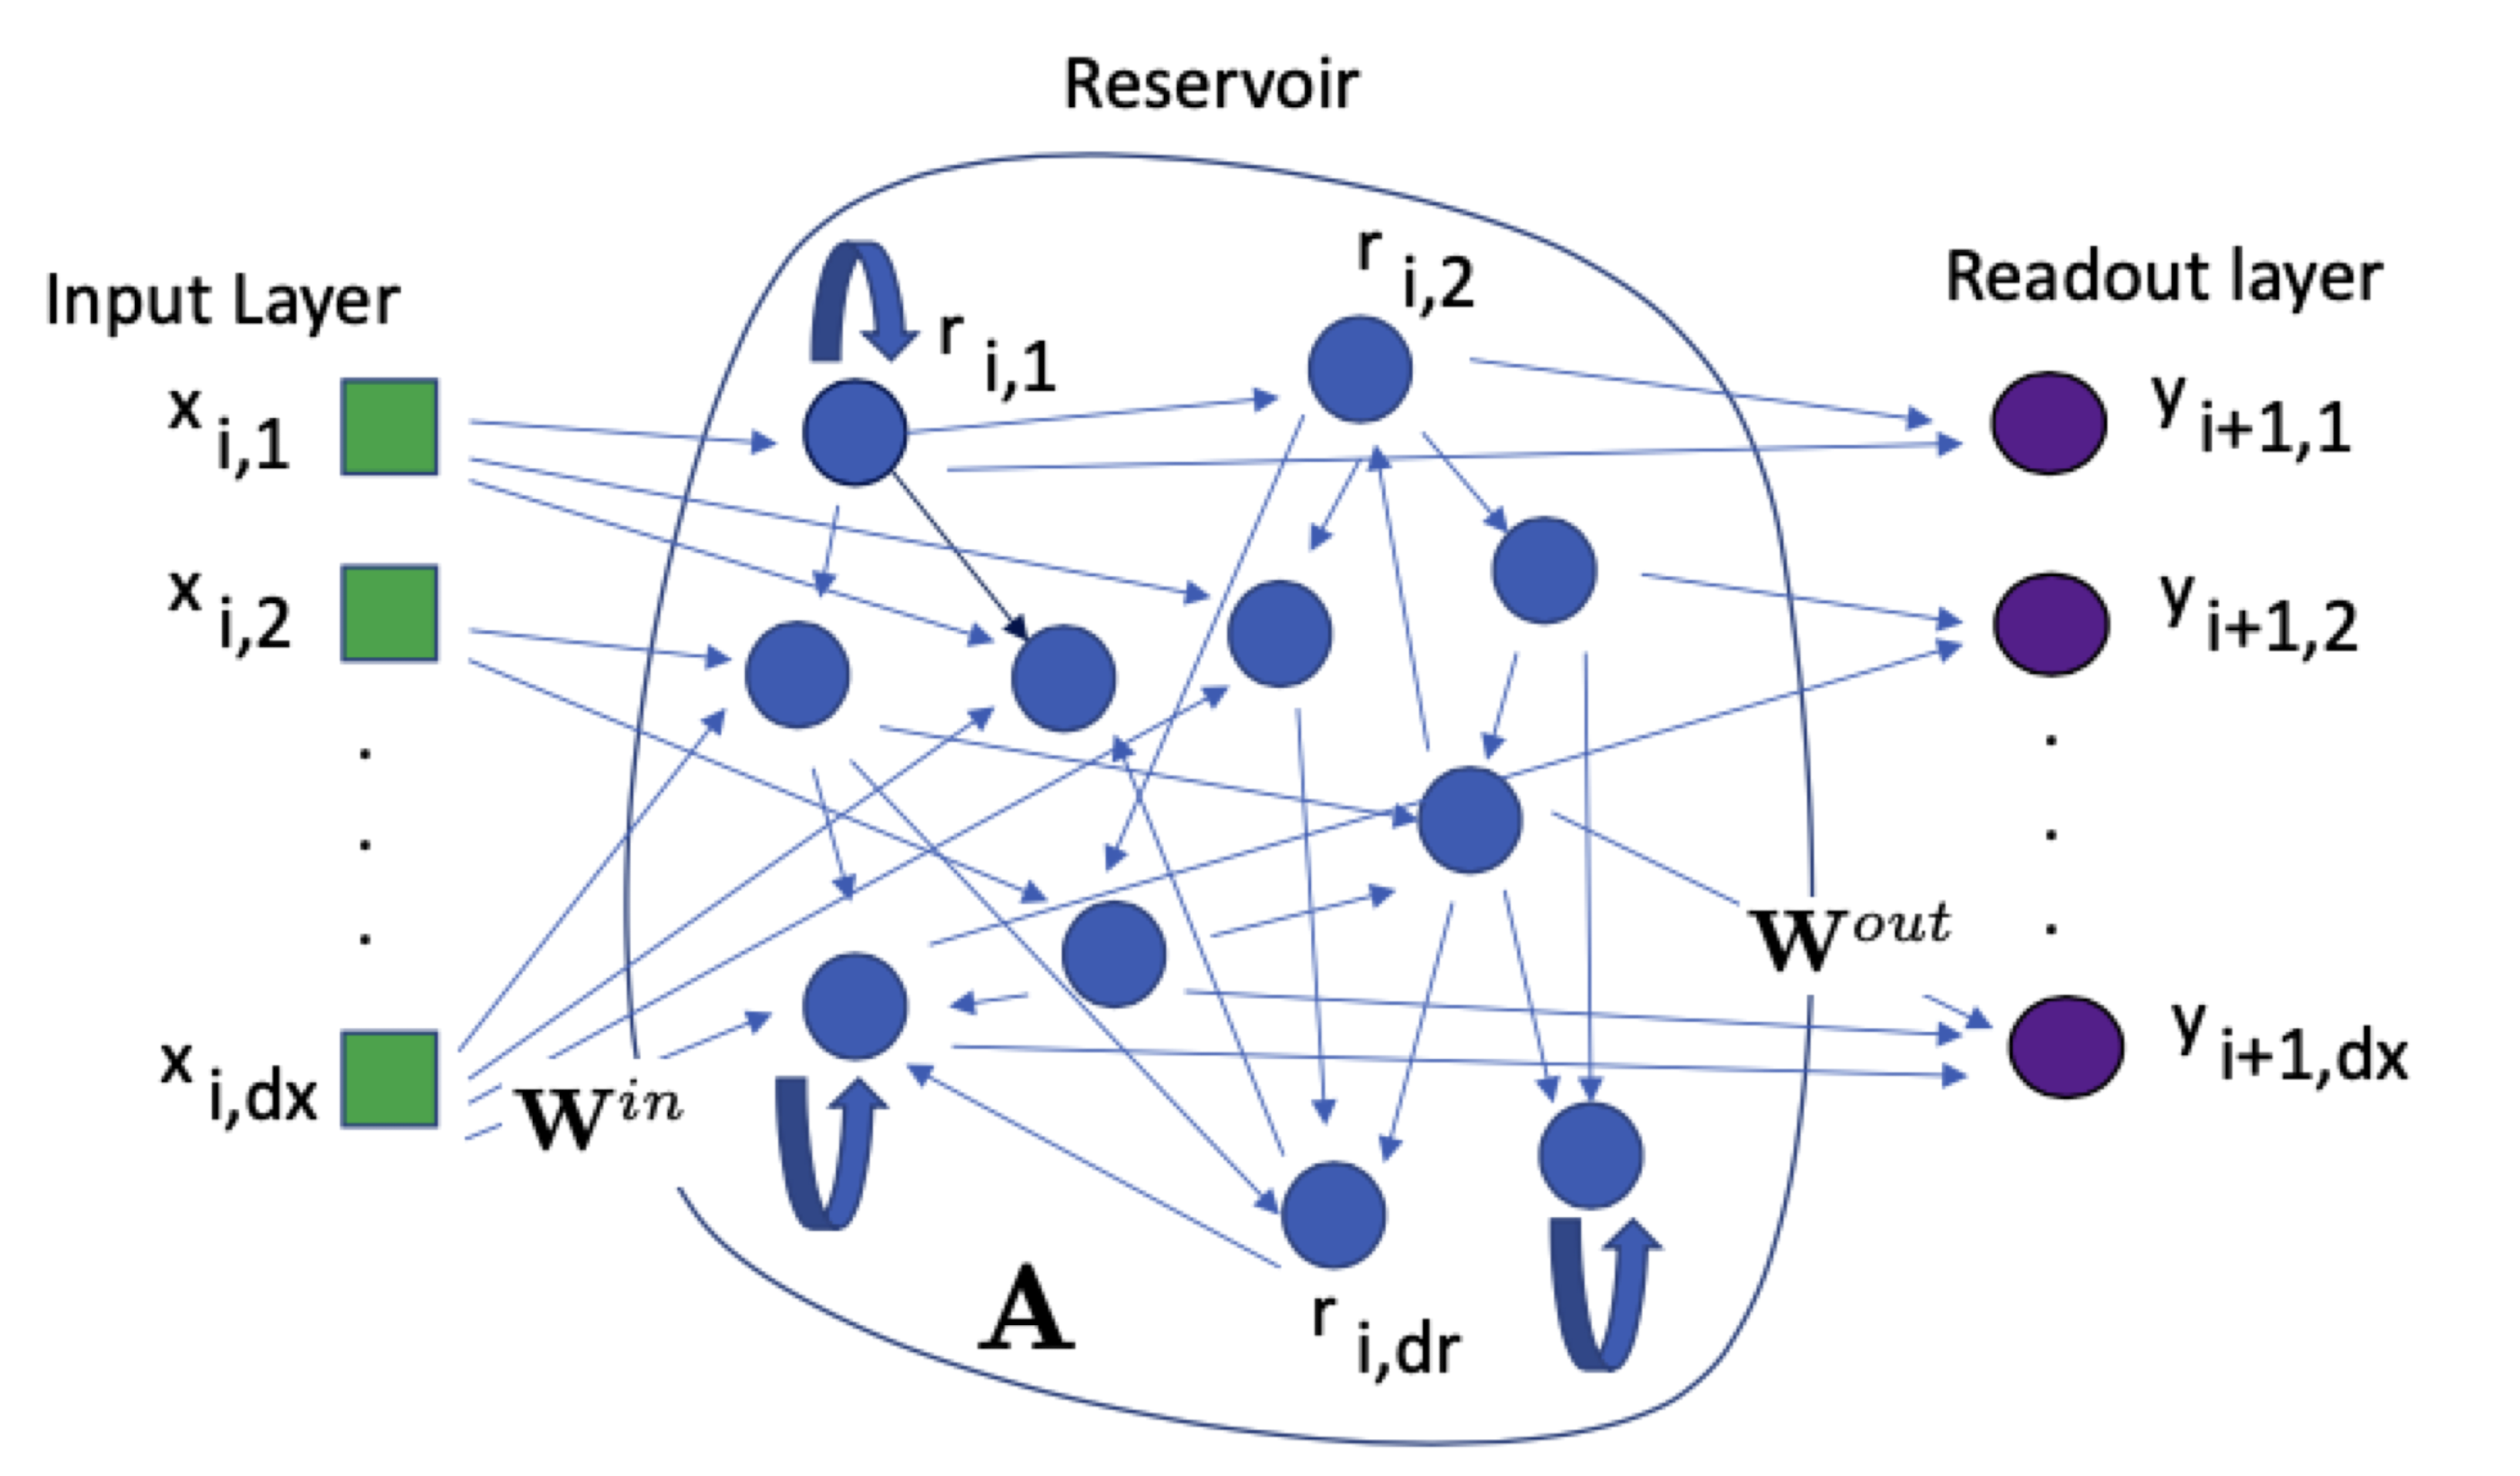
\includegraphics[width=\textwidth]{Fig/bollt_reservoir.png}
                \caption{\scriptsize{Reservoir Computer の各層の関係} \\ \tiny{Fig. 2 from \cite{Bollt}}}
            \end{figure}
        \end{column}
      \end{columns}
\end{frame}

\begin{frame}{Reservoir Computerの学習}
    \begin{itemize}
        \item Reservoir Computer の特徴は,出力層の行列 $\mathbf{W}^{\text {out }}$ のみ学習されること.\begin{itemize}
            \item 他の RNN では,$\mathbf{W}^{\text {in}}, \mathbf{A}$も学習の対象 
            
            \rightarrow 高次元空間の中で,非線形関数の $q(\cdot)$ の関わる勾配降下法最適化をしなければならない 
            
            \item Reservoir Computer はこれを回避し,$\mathbf{W}^{\text {out }}$の学習は線形な演算になる: 
            \begin{align}
                \mathbf{W}_{\text {out }}=\underset{\mathbf{V} \in \mathbb{R}^{d_x \times d_r}}{\arg \min }\|\underline{\mathbf{X}}-\mathbf{V R}\|_F=\underset{\mathbf{V} \in \mathbb{R}^{d_x \times d_r}}{\arg \min } \sum_{i=k}^N\left\|\mathbf{x}_i-\mathbf{V r}_i\right\|_2, k \geq 1 
            \end{align}
            $k > 1$ で Reservoir Computer のメモリを反映させることができる.
            \item Ridge Regression(リッジ回帰)、またはTikhonov正則化を伴う最小二乗法を用いて,過学習を防ぎながら学習させる(Hyperparameter の ridge については後述).解は形式的に次のように表される:
            \begin{align}
                \mathbf{W}^{\text {out }}:=\mathbf{X R}^T\left(\mathbf{R R}^T+\lambda \mathbf{I}\right)^{-1}
            \end{align}
        \end{itemize}
    \end{itemize}
\end{frame}

\begin{frame}{備考:Ridge Regressionについて}
  \begin{columns}[T] % [T] は列を上部で揃えるオプション  
    \begin{column}{.5\textwidth}
      \begin{align}
        Y=\beta_0+\beta_1 X_1+\beta_2 X_2+\cdots+\beta_n X_n+\epsilon
      \end{align}
       と表される線形回帰モデルがあるとする.ただし,$Y$ は目的関数,$X_1, \ldots, X_n$ は説明変数,$\beta_1, \ldots, \beta_n$ は回帰係数,$\epsilon$ は誤差項.
       このとき,Ridge regression の損失関数 $L$ は
       \begin{align}
        L(\beta)=\|Y-X \beta\|^2+\lambda\|\beta\|^2 \label{ridge}
       \end{align}
       で表される\footnote{\tiny{\eqref{ridge}の第一項は最小二乗誤差,第二項は $L_2$ ノルム正則化.}}.損失関数に正則化項を追加し,回帰係数に対するペナルティを与えることで,モデルの過学習を防ぐ.
    \end{column}
    \begin{column}{.5\textwidth}
      \begin{block}{reservoirpy における RidgeRegression}
        \begin{itemize}
          \item reservoirpyでは次の式で表される.
          \begin{align}
            W_{\text {out }}=Y X^T \cdot\left(X X^T+{ }_{\text {ridge }} \times \operatorname{Id}_{d i m_i n}\right)
          \end{align}
          \item $X$ が reservoir の中の状態,$Y$ がターゲットとなるベクトル,$d i m_i n$ は reservoir の中の状態の次元( reservoir のunit 数と対応).
        \end{itemize}
      \end{block}
    
    \end{column}
  \end{columns}
\end{frame}

\subsection{Reservoir Computer に関する理論}
\begin{frame}{Reservoir Computer に対する理論的な研究}
    Reservoir Computer や RNN, Echo State Network (ESN) (いずれも Reservoir Computer が属している機械学習の枠組み)に関する,いくつかの理論的な先行研究をまとめた.
    \begin{block}{Reservoir Computer に関する理論的な考察}
      \begin{itemize}
        \item \cite{Berry}: ダイナミクスに関する包括的な学習理論を与える.埋め込みの概念を用いた枠組みを示し,delay-coordinates と reservoir computer を用いた二つの主な力学系学習パラダイムに対して共通の説明を行う.
        \item \cite{Bollt}: activation function $q(\cdot)$ が線形関数であるときの Reservoir Computer と Vector Autoregression (VAR) の関係を説明.
        \item \cite{Gregoryeva}: Takens の埋め込み定理の一般化を行い,Reservoir Computer との関係性を示す.
      \end{itemize}
    \end{block}
\end{frame}

\begin{frame}{Reservior Computer と Takens の埋め込み定理 \cite{Gregoryeva} (1/4)}
    Reservoir Computer に関する理論的な枠組みについて,特に\cite{Gregoryeva}の内容を一部紹介する.\cite{Gregoryeva}では,Takens の埋め込み定理の General synchronization に関わる形で一般化を行った上で,その事実を用いてReservoir Computer (ただし,出力が非線形であるという条件を課す)が特定のダイナミクスの
    \begin{enumerate}
      \item 限られた観測変数から情報を復元
      \item 予測
    \end{enumerate}
    という二つのタスクに関して性能を発揮する原理を説明する.

    Reservoir Computer を始めとする RNN や ESN は Takensの埋め込み定理に関連する特性を持つ.特に \cite{Hart_1}, \cite{Hart_2} では ESN がコンパクト多様体に対して一次元の観測を行えるとき,特定の条件のもとでもとの系と位相共役であるダイナミクスを作れることが示された.
\end{frame}

\begin{frame}{Reservior Computer と Takens の埋め込み定理 \cite{Gregoryeva} (2/4)}
  \cite{Gregoryeva}において,Takens の埋め込み定理は次の形で述べられている.
  \begin{block}{Theorem 1.1 (Takens)  from \cite{Gregoryeva}}
    Let $M$ be a compact manifold of dimension $q \in \mathbb{N}$ and let $\phi \in \operatorname{Diff}^2(M)$ be a twice-differentiable diffeomorphism that satisfies the following two properties:

    \begin{enumerate}
      \item $\phi$ has only finitely many periodic points with periods less than or equal to $2 q$.
    
      \item If $m \in M$ is any periodic point of $\phi$ with period $k<2 q$, then the eigenvalues of the linear map $T_m \phi^k: T_m M \longrightarrow T_m M$ are distinct.
    \end{enumerate}
    
    Then for any generic scalar observation function $\omega \in C^2(M, \mathbb{R})$, the $(2 q+1)$-delay map $\Phi_{(\phi, \omega)}: M \longrightarrow$ $\mathbb{R}^{2 q+1}$ defined by
    $$
    \Phi_{(\phi, \omega)}(m):=\left(\omega(m), \omega \circ \phi(m), \omega \circ \phi^2(m), \ldots, \omega \circ \phi^{2 q}(m)\right)
    $$
    is an embedding in $C^1\left(M, \mathbb{R}^{2 q+1}\right)$.
  \end{block}
\end{frame}

\begin{frame}{Reservior Computer と Takens の埋め込み定理 \cite{Gregoryeva} (3/4)}

  なお,\cite{Berry}では RNN と Takens の埋め込み定理を用いた力学系のrepresentationの方法を統一する枠組みとして generalized synchronization (GS) について述べている.Takens の埋め込み定理は GS の枠組みの中で Takensの埋め込み定理を定式化する.
  
  (途中は割愛するが)次頁の定理の証明によって,Reservoir と GS の意味での Takensの埋め込み定理 の間の関連を述べ,Reservoir の場合も埋め込みが得られることを述べている.
\end{frame}

\begin{frame}{Reservior Computer と Takens の埋め込み定理 \cite{Gregoryeva} (4/4)}
  \begin{block}{Theorem 4.5 (Linear reservoir embeddings) from \cite{Gregoryeva}}
     Let $\phi \in \operatorname{Diff}^2(M)$ be a dynamical system on a compact manifold $M$ of dimension $q$ that exhibits finitely many periodic orbits. Suppose that for each periodic orbit $m$ of $\phi$ with period $n \in \mathbb{N}$, the derivative $T_m \phi^{-n}$ has $q$ distinct eigenvalues $\lambda_1, \lambda_2, \ldots, \lambda_q$. Let now $\ell \in \mathbb{N}$ be the lowest common multiple of all the periods of the finite periodic points of $\phi$ and let $N \in \mathbb{N}$ such that $N>\max \{2 q, \ell\}$.

Construct now $\bar{A} \in \mathbb{M}_{N, N}$ and $\overline{\mathbf{C}} \in \mathbb{R}^N$ by drawing their entries using independent regular realvalued distributions. Then, there exist rescaled versions $A$ and $\mathbf{C}$ of $\bar{A}$ and $\overline{\mathbf{C}}$ respectively such that the generalized synchronization $f_{(\phi, \omega, F)} \in C^2(M, \mathbb{R})$ associated to the state map $F(\mathbf{x}, z):=A \mathbf{x}+\mathbf{C} z$ is almost surely an embedding for generic $\omega \in C^2\left(M, \mathbb{R}^N\right)$.
  \end{block}
\end{frame}

\subsection{実験に関する先行研究}



\begin{frame}{Y. C. Lai et al. (2022) の結果 (1/2)}
    ここでは,実験面での先行研究として,\cite{Kong}について触れる.
    \begin{block}{Reservior Computer の構成:Y. C. Lai et al. (2022)}
    \vspace{0.1cm}
        \begin{minipage}{0.4\textwidth}
            \begin{figure}
                %\centering % 画像を中央揃えにする(オプション)
                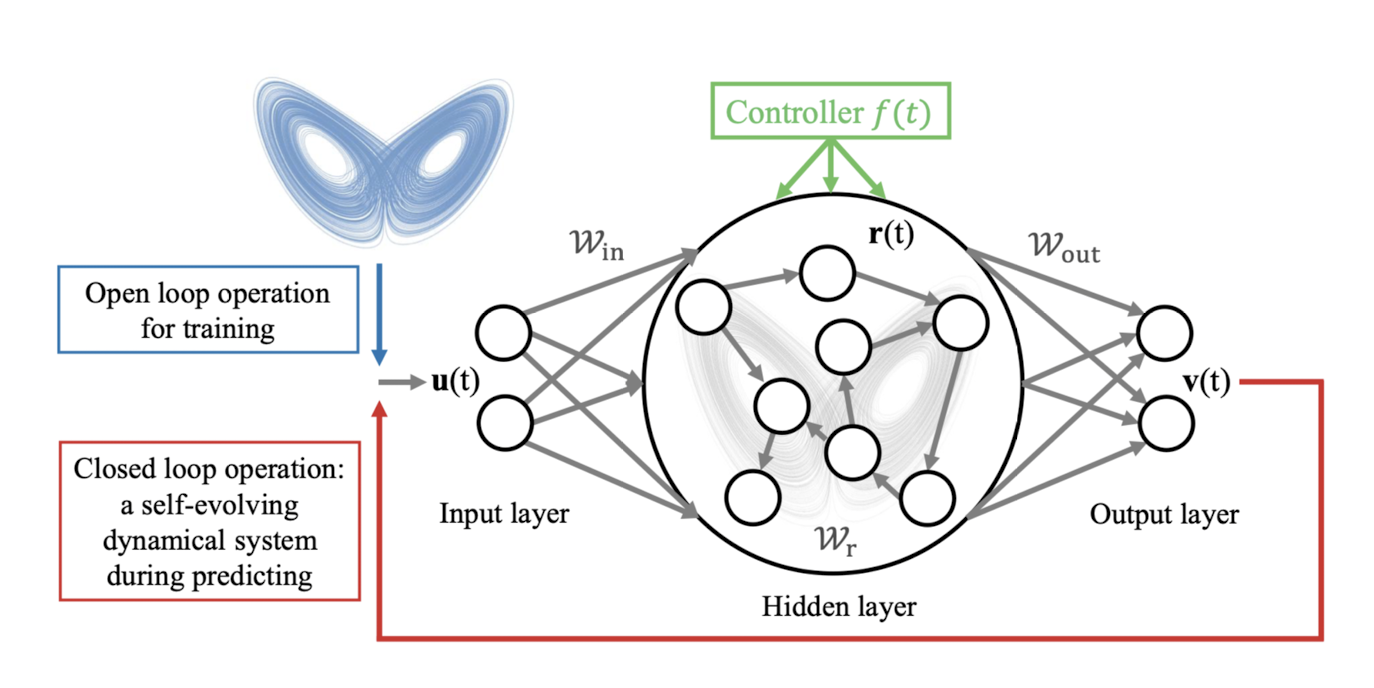
\includegraphics[width=\textwidth]{Fig/Fig.1_Lai.png}
                \caption*{Fig.1 from Y. C. Lai et al. (2022)}
                \label{Fig.1_Lai.png} % ラベルを付ける(参照する場合に使用)
            \end{figure}
        \end{minipage}%
        \begin{minipage}{0.6\textwidth}
            \begin{itemize}
                \item $\mathbf{u}(t) \in \R^{D_{\text{in}}}$: input signal. 
                \item $\mathbf{r}(t) \in \R^{D_r} $: hidden layer state vector.
                \item $f(t)$: (control) external driving signal.  
                \item $\mathcal{W}_{\text{in}} \in D_r \times D_{\text{in}}$: Weighted input matrix.  
                \item $\mathcal{W}_c$: Controller matrix.
                \item $ \mathcal{W}_r \in D_r \times D_{r}$: Weighted network matrix inside.
                \item $\mathcal{W}_{\text{out}}: D_{\text{out}} \times D_{r}$: Output weighted matrix.
            \end{itemize}
    \end{minipage}
    \end{block}
    $\mathbf{u}(t)$ に時系列モデル(low/high-dimensional Lorenz-96 climate network, driven chaotic laser systemなど),$f(t)$にはsinusoidal関数などを使用する(e.g. $f(t) = A \sin (\Omega t) + F$).
\end{frame}

\begin{frame}{Y. C. Lai et al. (2022) の結果 (2/2)}
    学習期間全体の $\mathbf{u}(t)$,全期間の $\mathbf{v}(t)$ を記録する行列をそれぞれ $\mathcal{R'}, \mathcal{V}$ とする.
    \begin{itemize}
        \item $\mathcal{W}_{\text {in }}, \mathcal{W}_c, \mathcal{W}_r$ は Reservior の学習に前もってランダムに定められる.
        \item 学習期間において,$\mathbf{u(t)}$ と $f(t)$ の実データが入力される.
        学習期間の後のself-evolving 期間では,Reservior による出力 $\mathbf{v}(t)$ と $f(t)$ の実データが予測の入力に用いられる.
        \begin{itemize}
            \item $\mathbf{r}(t)$ は 学習期間,self-evolving 期間においてそれぞれ次の式で決定される.
            \vspace{-.2cm}
            \begin{align}
                \mathbf{r}(t+\Delta t) & =(1-\alpha) \mathbf{r}(t) + \alpha \tanh \left[\mathcal{W}_r \mathbf{r}(t)+\mathcal{W}_{\text {in }} \mathbf{u}(t)+\mathcal{W}_c f(t)\right] \label{Lai_r1}\\
                \mathbf{r}(t+\Delta t) & =(1-\alpha) \mathbf{r}(t) + \alpha \tanh \left[\mathcal{W}_r \mathbf{r}(t)+\mathcal{W}_{\text {in }} \mathcal{W}_{\text {out }} \mathbf{r}^{\prime}(t)+\mathcal{W}_c f(t)\right]\label{Lai_r2}
            \end{align}
        \end{itemize}
        \item 複数の $f(t)$ に対して Reservior を sequential に学習させることで,未知の外力がある場合でも予測できるようにする.また,Hyperparameter に関する最適化を行う(後述).
        \item Reservoir に次式における$\mathcal{V}, \mathcal{R'}$ 間のLinear Regressionを通じて$\mathcal{W}_{\text {out }}$ を学習させる.
        \vspace{-.2cm}
        \begin{align}
            \mathcal{W}_{\text {out }}=\mathcal{V} \cdot \mathcal{R}^{\prime T}\left(\mathcal{R}^{\prime} \cdot \mathcal{R}^{\prime T}+\beta \mathcal{I}\right)^{-1}
        \end{align}
    \end{itemize}

\end{frame}


\subsection{Hyperparameters の最適化}
\begin{frame}{Reservoir に関する Hyperparameters}
    Reservoir に関する Hyperparameter のうち,最適化の対象としたものを記した.説明は,\cite{rpy_doc}の Tutorial 4 を参考にした.
    \begin{enumerate}
        \item Cell Number (N): units, セル数.
        \item spectral radius (sr): スペクトル半径.Reservoir の 行列 $\mathcal{W}$ の固有値の絶対値の最大値.\begin{itemize}
            \item 小さいと安定したダイナミクス、大きいとカオス的なダイナミクス.
            \item 理論的には$1$ に近いと Reservoir の初期条件に影響を受けにくく,良好な memory を持つことが推測される.
        \end{itemize}
        \item input scaling (iss): Reservoir の入力 $\mathcal{W}_{in}$ に適用される係数.入力にゲインを加える.\begin{itemize}
            \item 高くするとReservoir と 入力の相関を(飽和点まで)高める.
            \item 低くすると Reservoir は外部の入力より自身のダイナミクスに強く影響を受ける.
            \item 多変量時系列データの各変数の影響度を調整可能.
        \end{itemize}
        \item leaking rate (lr): 次ステップの決定に際しての現在の状態と新しい入力の影響度の割合.\begin{itemize}
            \item 高い(低い)と惰性が高く(低く),過去の記憶状態が高く(低く)なる.
            \item ESN のネットワークがその状態を変化させる速度を制御する.
        \end{itemize}
        \item ridge (ridge): ridge regression における 正則化パラメータ.$0$ の時,ridge regression の結果は擬似行列を使った解と一致する.
    \end{enumerate}
\end{frame}

\begin{frame}{Hyperparameters 最適化のアルゴリズム}
    Hyperparameters の最適化には python ライブラリである Optuna を用いた.
     
    Optunaで実装されている Hyperparameters の最適化アルゴリズムは例えば以下がある.
    \begin{columns}[T] % [T] は列を上部で揃えるオプション
        \begin{column}{.5\textwidth}
            

            \begin{block}{optuna.samplers: from \cite{optuna_doc}}
                \begin{enumerate}
                    \item \textbf{optuna.samplers.RandomSampler}: ランダムサンプリングを使用するサンプラー。
                    \item \textbf{optuna.samplers.TPESampler}: TPE(Tree-structured Parzen Estimator)アルゴリズムを使用するサンプラー。
                    \item \textbf{optuna.samplers.CmaEsSampler}: CMA-ES(Covariance Matrix Adaptation Evolution Strategy)をバックエンドとして使用するサンプラー。
                \end{enumerate}
                
            \end{block}
        
        \end{column}
        \begin{column}{.5\textwidth}
            \begin{itemize}
                \item この研究では,CmaEsSampler (最終的に採用), TPESampler と hyperopt という別のpython ライブラリの random search を用いた.\begin{itemize}
                    \item 経験的に,同順により好ましい best value を与えた.
                    
                \end{itemize}
                \item また,Optuna搭載の pruner も利用した.\begin{itemize}
                    \item 見込みの悪い Hyperparameters のセットを見限ること.
                    \item 使用したのは SuccessiveHalvingPruner.
                \end{itemize}
                \item なお,hyperopt には Optunaのいくつかの機能は搭載されていないので注意.
            \end{itemize}
        \end{column}
      \end{columns}


\end{frame}


\subsection{実験のパラメータ設定}

\begin{frame}
    \begin{columns}[T] % [T] は列を上部で揃えるオプション
        \begin{column}{.5\textwidth}
            \begin{itemize}
                \item Rössler系の数値シミュレーション\begin{itemize}
                    \item $A = 1.0$ 
                    \item $a = 0.2,\ b = 0.2,\ c = 5.7.$ 
                    \item 初期条件:$\left[ X_0, Y_0, Z_0 \right] = [1.0, 1.0, 1.0]$ 
                    \item 時間範囲:$t_\text{span} = [0, 4510].$ 
                    \item 位相シフト時間:$p = 8$ に対して Hyperparameter を最適化. 
                    \item 注.配列データは $1$ タイムステップに対して $10$ 個データポイントをとって生成したので,長さ $[0, 45100]$ である.
                \end{itemize}
                \item Optunaの最適化
                \begin{itemize}
                    \item $\text{nb seeds} = 3$
                    \item $\text{nb trials} = 3000$ 
                    \item 最適化アルゴリズム:CmaEsSampler
                    \item pruner: SuccessiveHalvingPruner
                    \item $\text{train len} = 20000$
                    \item $\text{test len} = 10000$
                \end{itemize}
            \end{itemize}
        \end{column}
        \begin{column}{.5\textwidth}
            \begin{itemize}
                \item Hyperparameters の探索空間\begin{itemize}
                    \item N = 10000: 固定

                    sr:  (1e-2, 10, log = True)

                    lr: (1e-3, 1, log = True)

                    iss: (0, 1)
                    
                    ridge: (1e-9, 1e-2, log = True)

                    \item 一様ランダムにサンプリング.
                    \item log = True で$\log$ をとって一様ランダムにサンプリング.
                \end{itemize}
                \item 採用した Hyperparameters のセット\begin{itemize}
                    \item Best value: 0.0017332259260817507
                    Best parameters: {
                        
                        'sr': 0.568437354122632, 
                        
                        'lr': 0.33989147591891816, 
                        
                        'iss': 0.08827385538440446, 
                        
                        'ridge': 1.30084237042553e-08}
                \end{itemize}
            \end{itemize}
        \end{column}
      \end{columns}
    
\end{frame}

\subsection{結果のまとめ}
\begin{frame}{self-evolve 期間における予測結果:位相シフトが$8, 10$のとき(再掲)}
    \begin{columns}[T] % [T] は列を上部で揃えるオプション
      \begin{column}{.5\textwidth}
        \begin{figure}
          \vspace{-.5cm}
          % 画像1
          \begin{minipage}[c][.27\textheight][c]{\linewidth}
            \centering
            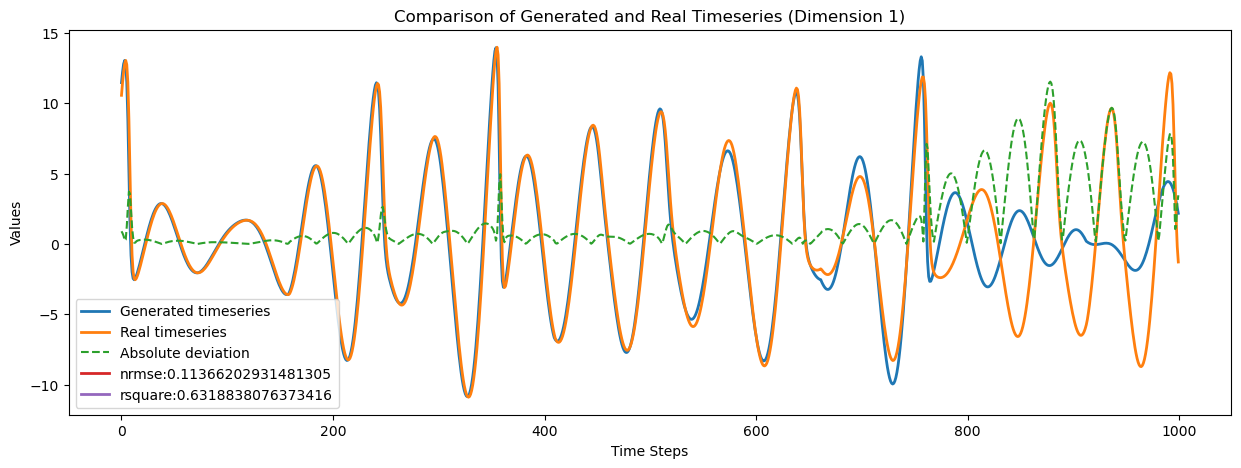
\includegraphics[width=0.7\linewidth]{Fig/8.x.png}
          \end{minipage}
      
          \vspace{-.5em}
  
          % 画像2
          \begin{minipage}[c][.27\textheight][c]{\linewidth}
            \centering
            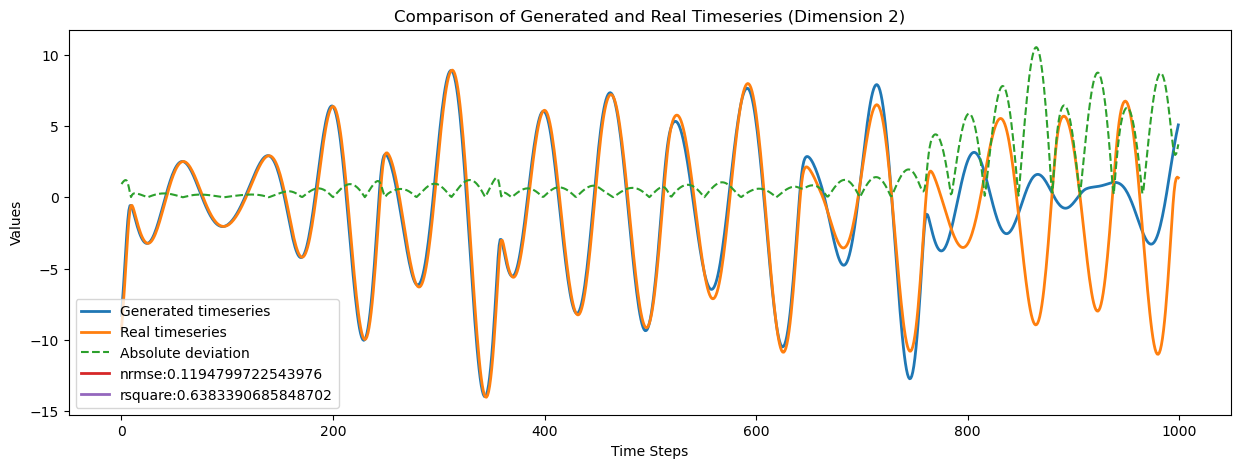
\includegraphics[width=0.7\linewidth]{Fig/8.y.png}
          \end{minipage}
          
          \vspace{.5em}
          % 画像3
          \begin{minipage}[c][.27\textheight][c]{\linewidth}
            \centering
            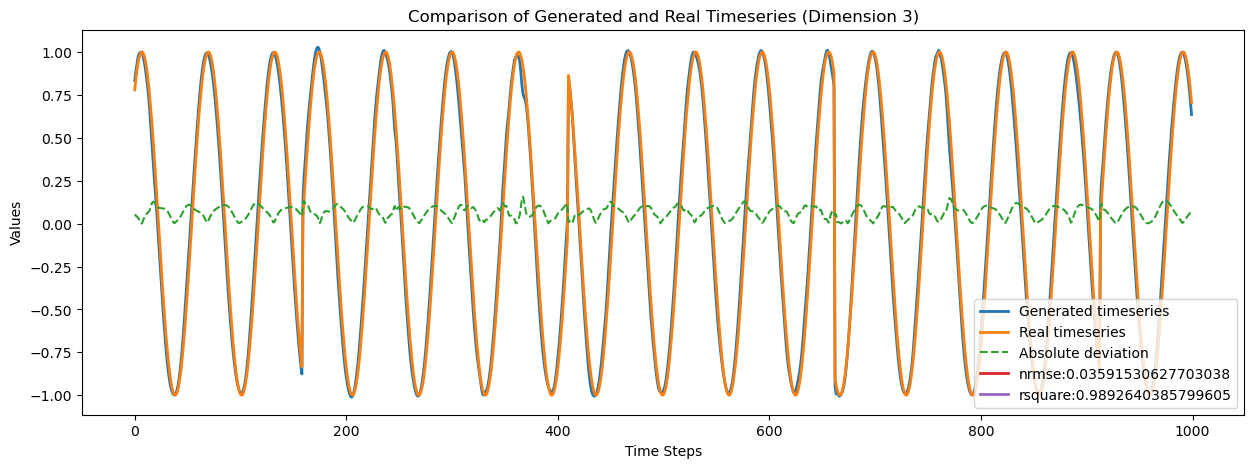
\includegraphics[width=0.7\linewidth]{Fig/8.p.png}
            \caption{\scriptsize{位相シフト(8時間分)のある外力付きRösslerモデルの予測.上から $x, y, P(t)$. }}
          \end{minipage}
        \end{figure}
      \end{column}
      \begin{column}{.5\textwidth}
        \begin{figure}
          \vspace{-.5cm}
          % 画像1
          \begin{minipage}[c][.27\textheight][c]{\linewidth}
            \centering
            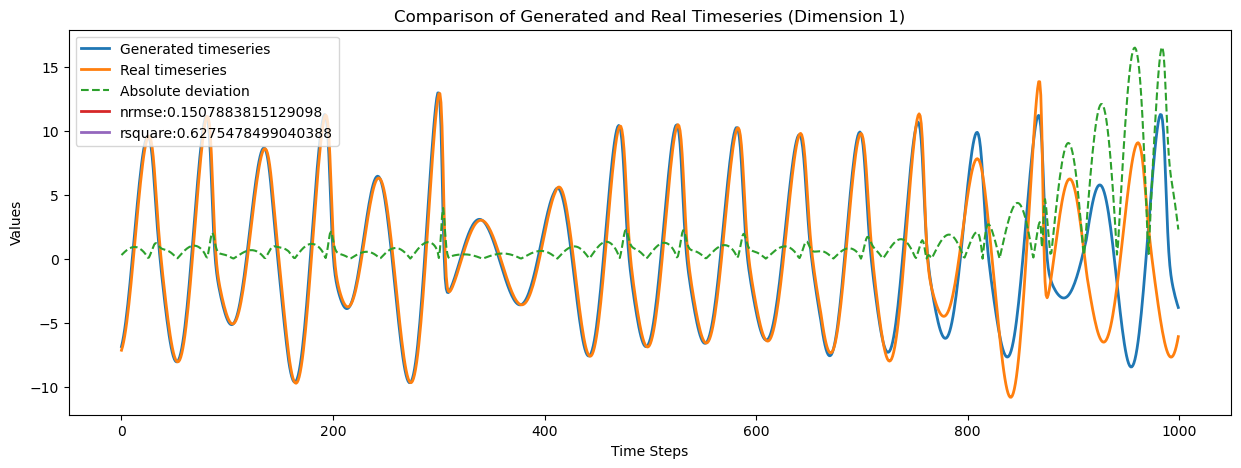
\includegraphics[width=0.7\linewidth]{Fig/10.x.png}
          \end{minipage}
      
          \vspace{-.5em}
  
          % 画像2
          \begin{minipage}[c][.27\textheight][c]{\linewidth}
            \centering
            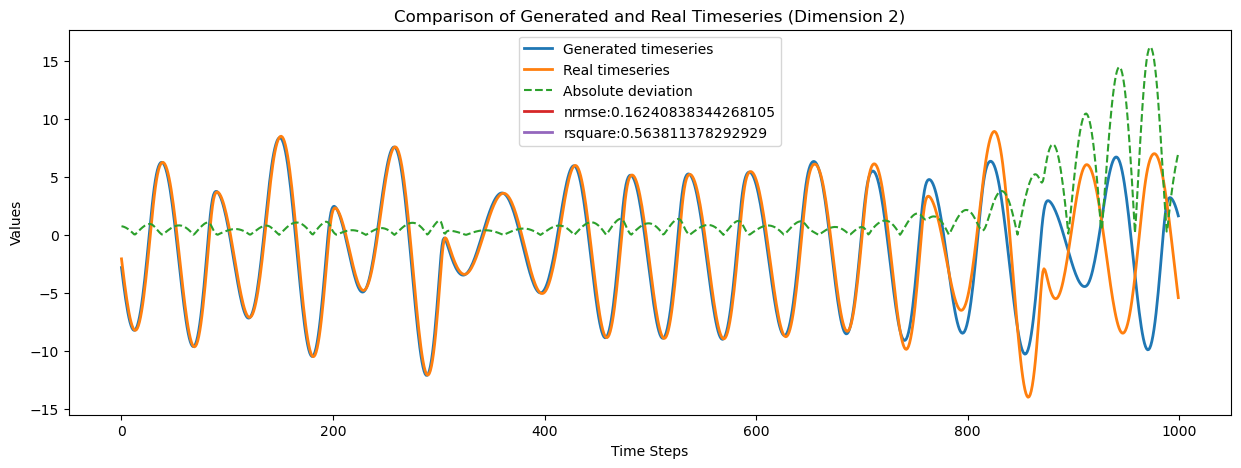
\includegraphics[width=0.7\linewidth]{Fig/10.y.png}
          \end{minipage}
          
          \vspace{.5em}
          % 画像3
          \begin{minipage}[c][.27\textheight][c]{\linewidth}
            \centering
            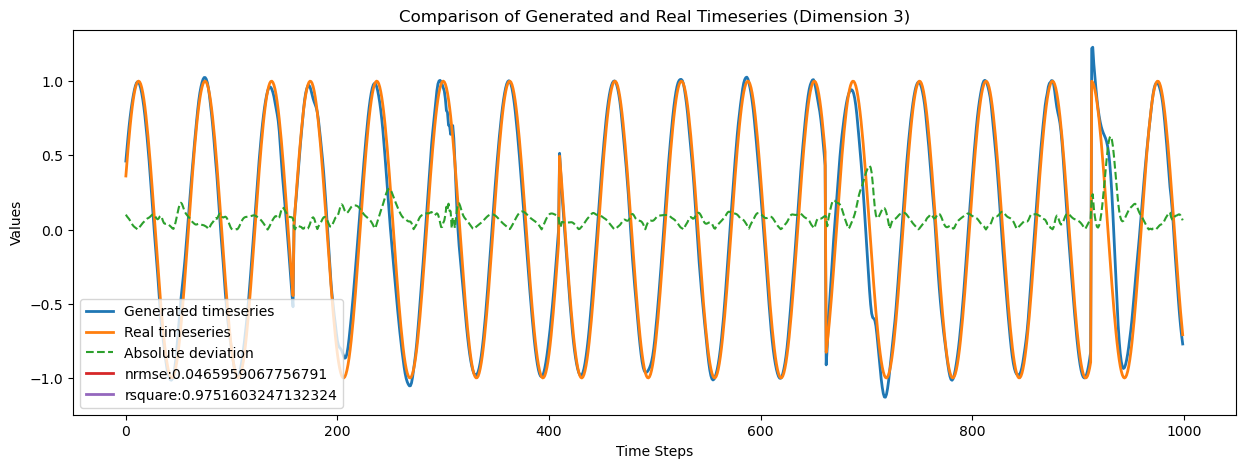
\includegraphics[width=0.7\linewidth]{Fig/10.p.png}
            \caption{\scriptsize{位相シフト(10時間分)のある外力付きRösslerモデルの予測.上から $x, y, P(t)$.}}
          \end{minipage}
        \end{figure}
      \end{column}
    \end{columns}
  \end{frame}

  \begin{frame}{self-evolve 期間における予測結果:位相シフトが$4, 6$のとき}
  \begin{columns}[T] % [T] は列を上部で揃えるオプション
    \begin{column}{.5\textwidth}
        \begin{figure}
            \vspace{-.5cm}
            % 画像1
            \begin{minipage}[c][.27\textheight][c]{\linewidth}
              \centering
              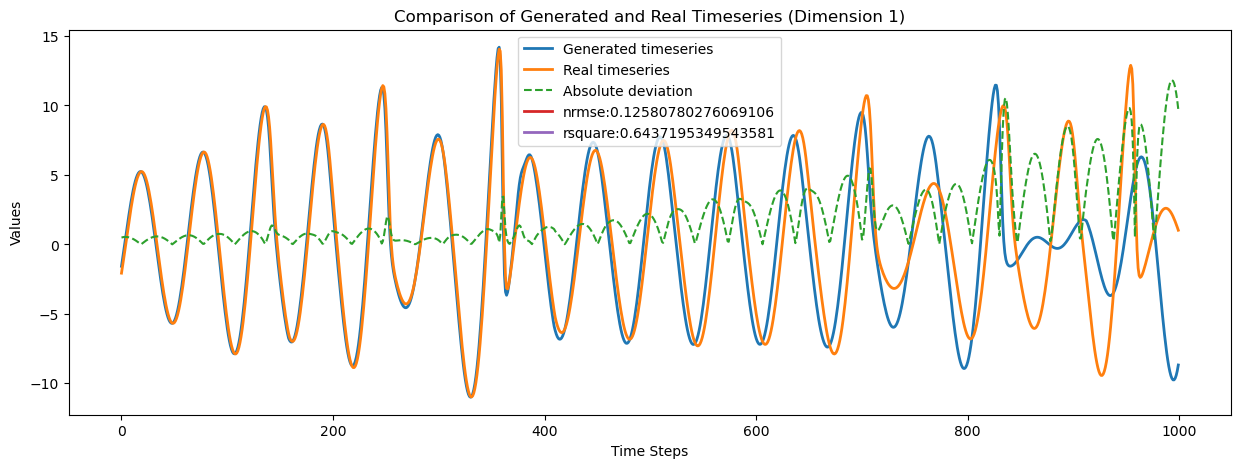
\includegraphics[width=0.7\linewidth]{Fig/4.x.png}
            \end{minipage}
        
            \vspace{-.5em}
    
            % 画像2
            \begin{minipage}[c][.27\textheight][c]{\linewidth}
              \centering
              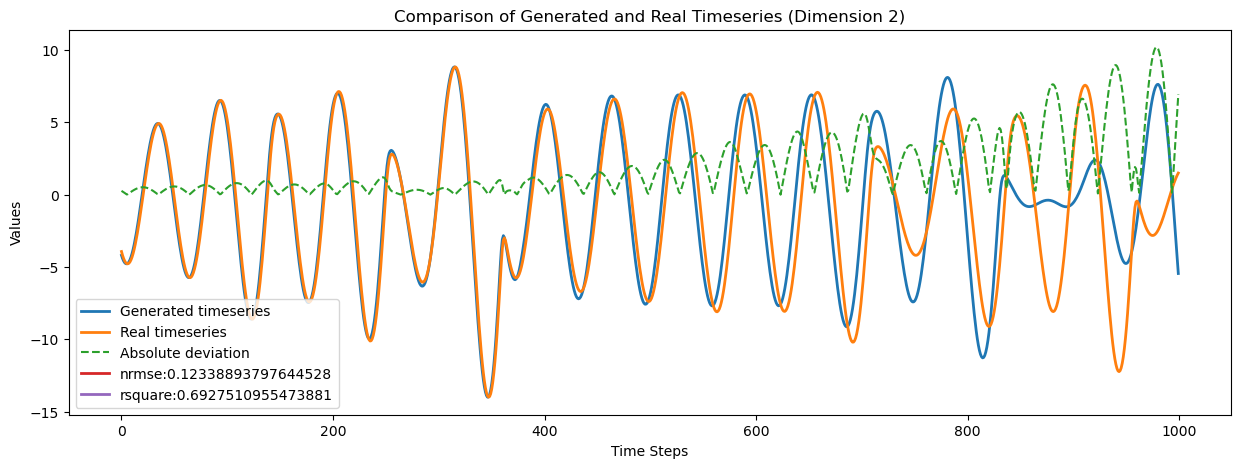
\includegraphics[width=0.7\linewidth]{Fig/4.y.png}
            \end{minipage}
            
            \vspace{.5em}
            % 画像3
            \begin{minipage}[c][.27\textheight][c]{\linewidth}
              \centering
              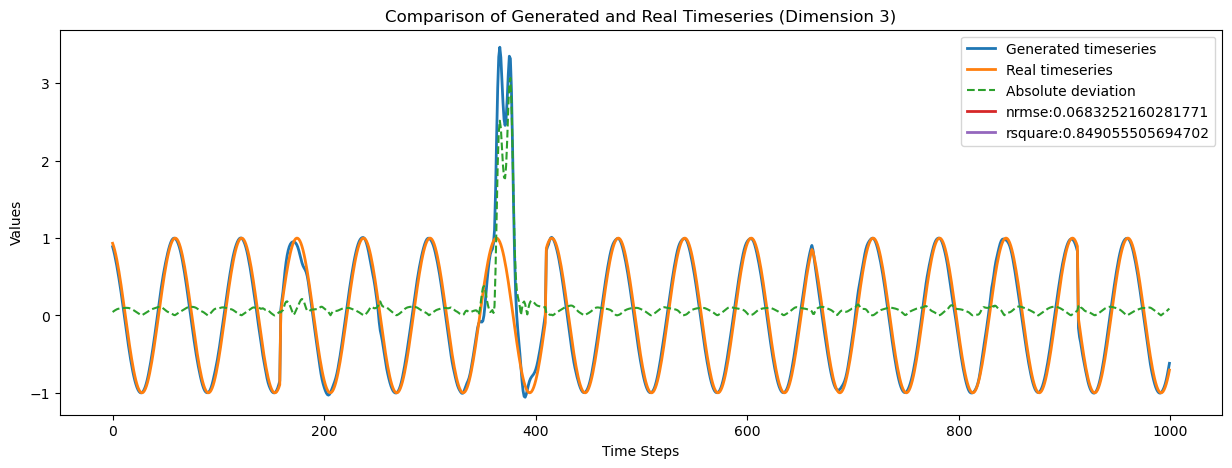
\includegraphics[width=0.7\linewidth]{Fig/4.p.png}
              \caption{\scriptsize{位相シフト(4時間分)のある外力付きRösslerモデルの予測.上から $x, y, P(t)$. }}
            \end{minipage}
          \end{figure}

    \end{column}
    \begin{column}{.5\textwidth}
      \begin{figure}
        \vspace{-.5cm}
        % 画像1
        \begin{minipage}[c][.27\textheight][c]{\linewidth}
          \centering
          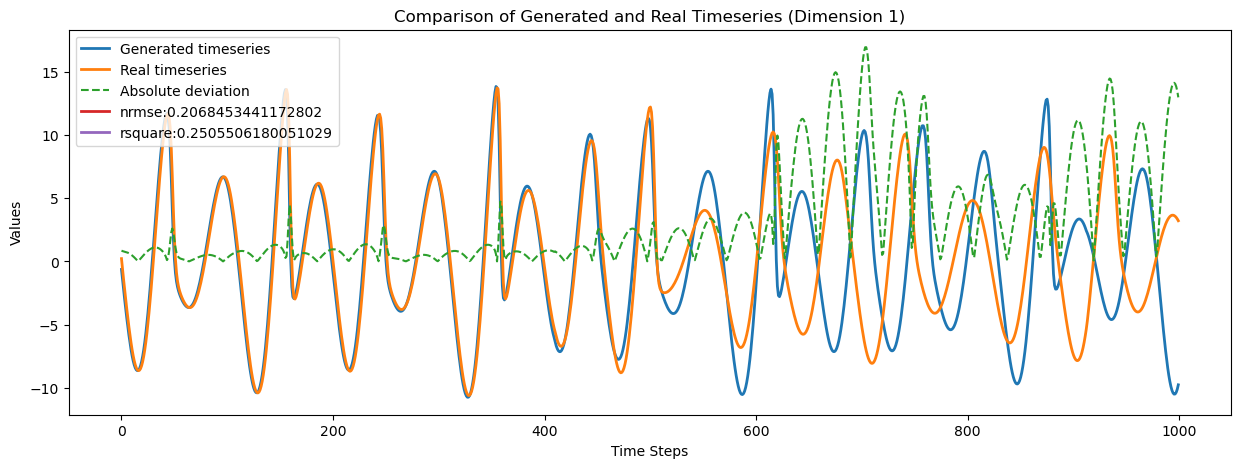
\includegraphics[width=0.7\linewidth]{Fig/6.x.png}
        \end{minipage}
    
        \vspace{-.5em}

        % 画像2
        \begin{minipage}[c][.27\textheight][c]{\linewidth}
          \centering
          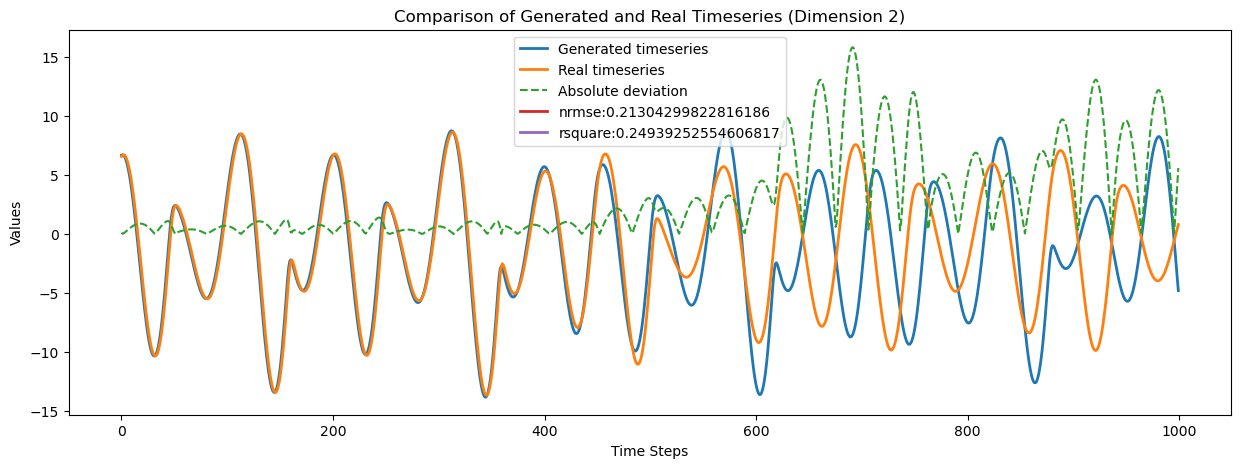
\includegraphics[width=0.7\linewidth]{Fig/6.y.png}
        \end{minipage}
        
        \vspace{.5em}
        % 画像3
        \begin{minipage}[c][.27\textheight][c]{\linewidth}
          \centering
          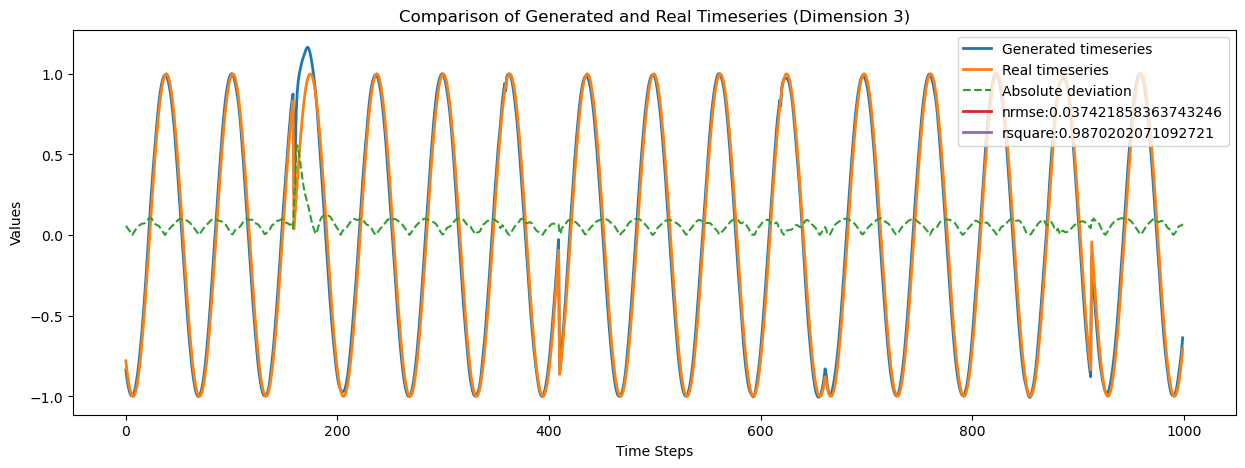
\includegraphics[width=0.7\linewidth]{Fig/6.p.png}
          \caption{\scriptsize{位相シフト(6時間分)のある外力付きRösslerモデルの予測.上から $x, y, P(t)$.}}
        \end{minipage}
      \end{figure}
    \end{column}
  \end{columns}
\end{frame}

\begin{frame}{self-evolve 期間における予測結果:位相シフトが$-4, -8$のとき}
    \begin{columns}[T] % [T] は列を上部で揃えるオプション
      \begin{column}{.5\textwidth}
        \begin{figure}
            \vspace{-.5cm}
            % 画像1
            \begin{minipage}[c][.27\textheight][c]{\linewidth}
              \centering
              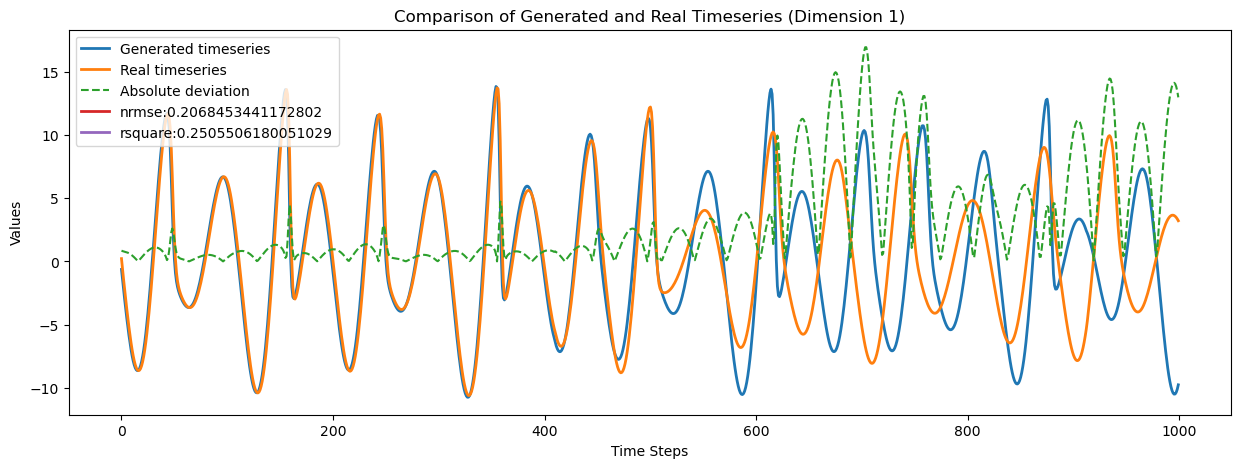
\includegraphics[width=0.7\linewidth]{Fig/-4.x.png}
            \end{minipage}
        
            \vspace{-.5em}
    
            % 画像2
            \begin{minipage}[c][.27\textheight][c]{\linewidth}
              \centering
              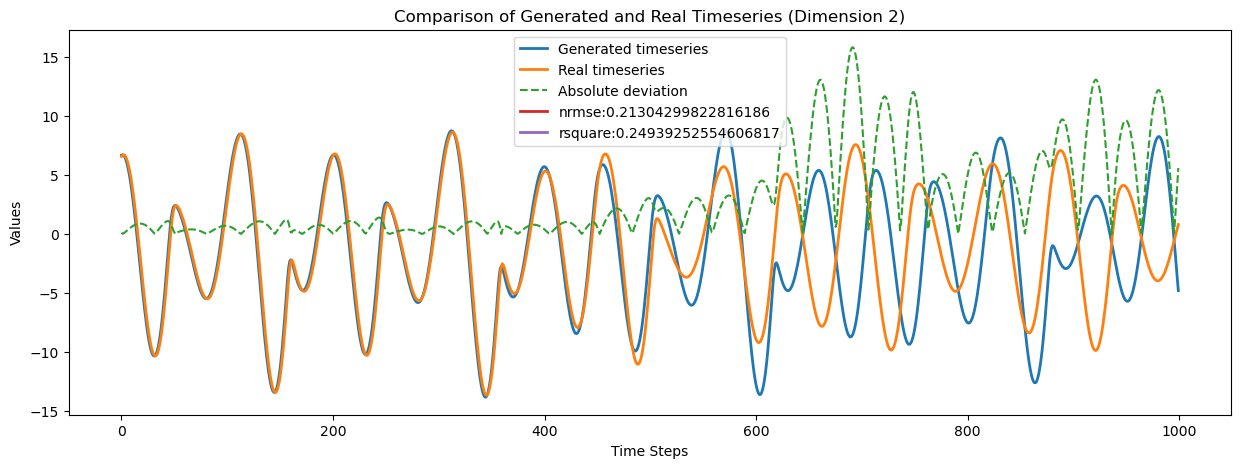
\includegraphics[width=0.7\linewidth]{Fig/-4.y.png}
            \end{minipage}
            
            \vspace{.5em}
            % 画像3
            \begin{minipage}[c][.27\textheight][c]{\linewidth}
              \centering
              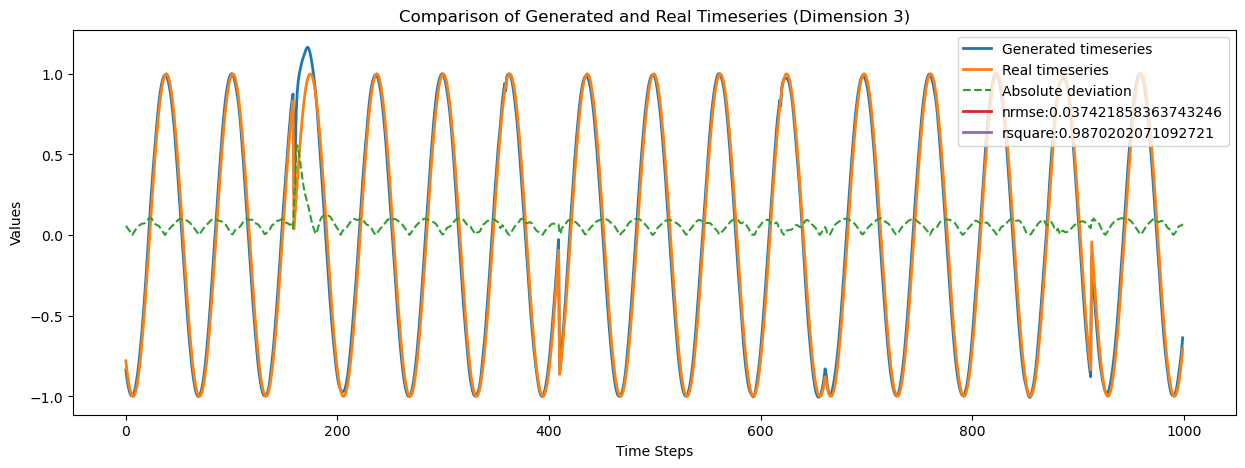
\includegraphics[width=0.7\linewidth]{Fig/-4.p.png}
              \caption{\scriptsize{位相シフト(-4時間分)のある外力付きRösslerモデルの予測.上から $x, y, P(t)$. }}
            \end{minipage}
          \end{figure}
      \end{column}
      \begin{column}{.5\textwidth}
        \begin{figure}
          \vspace{-.5cm}
          % 画像1
          \begin{minipage}[c][.27\textheight][c]{\linewidth}
            \centering
            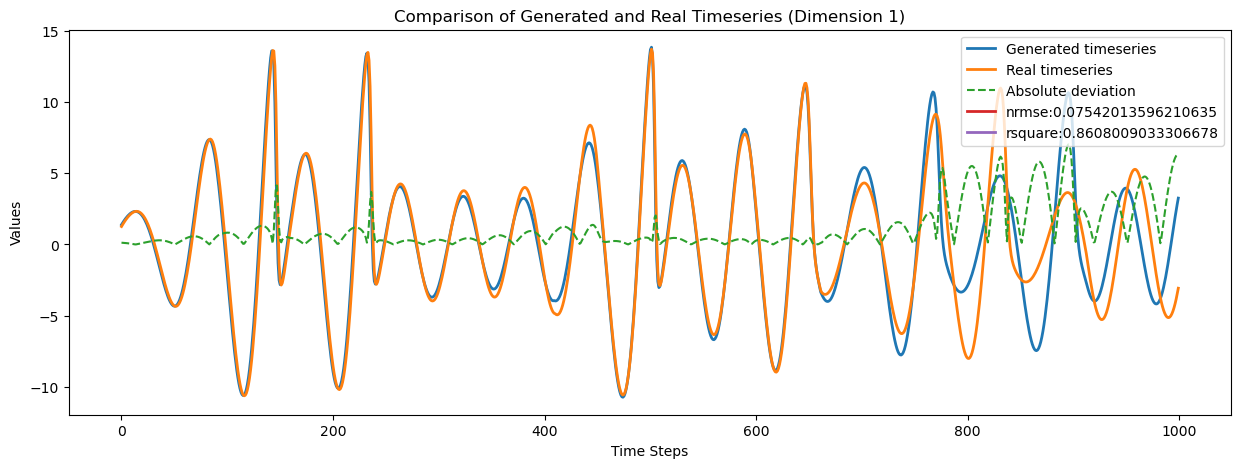
\includegraphics[width=0.7\linewidth]{Fig/-8.x.png}
          \end{minipage}
      
          \vspace{-.5em}
  
          % 画像2
          \begin{minipage}[c][.27\textheight][c]{\linewidth}
            \centering
            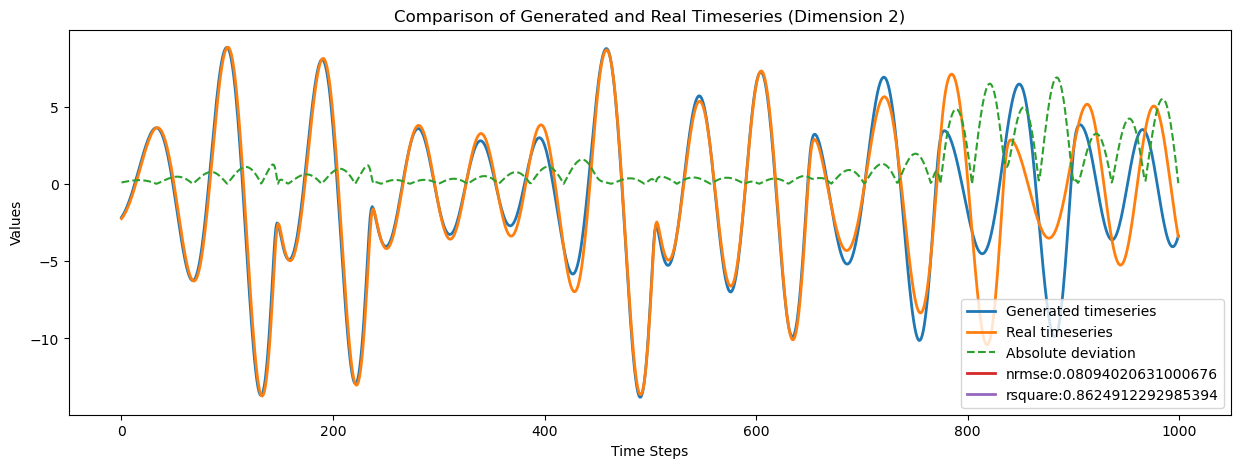
\includegraphics[width=0.7\linewidth]{Fig/-8.y.png}
          \end{minipage}
          
          \vspace{.5em}
          % 画像3
          \begin{minipage}[c][.27\textheight][c]{\linewidth}
            \centering
            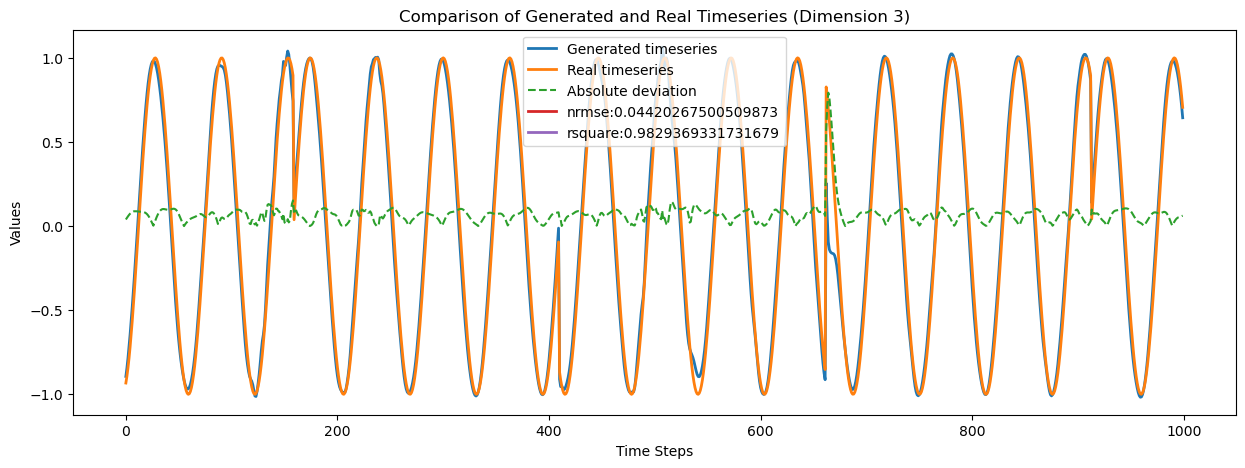
\includegraphics[width=0.7\linewidth]{Fig/-8.p.png}
            \caption{\scriptsize{位相シフト(-8時間分)のある外力付きRösslerモデルの予測.上から $x, y, P(t)$.}}
          \end{minipage}
        \end{figure}
      \end{column}
    \end{columns}
  \end{frame}
  
  



\section{参考文献}

\begin{frame}{参考文献 - 1}
    \begin{thebibliography}{99}    
        \bibitem[1]{Berry}
        Berry, T., and Das, S. (2023). Learning Theory for Dynamical Systems. SIAM Journal on Applied Dynamical Systems, 22(3), 2082–2122. \url{https://doi.org/10.1137/22M1516865}.
  
      
        \bibitem[2]{Bollt}
        Bollt, E.M. (2020). On explaining the surprising success of reservoir computing forecaster of chaos? The universal machine learning dynamical system with contrast to VAR and DMD. Chaos, 31 1, 013108 .

        
        
        \bibitem[3]{Gregoryeva}
        Grigoryeva, Lyudmila, Hart, Allen and Ortega, Juan-Pablo. (2023). Learning strange attractors with reservoir systems. Nonlinearity. 36. 10.1088/1361-6544/ace492.
    \end{thebibliography}
\end{frame}

\begin{frame}{参考文献 - 2}
  \begin{thebibliography}{99}    
      \bibitem[4]{Hart_1}
      A. G. Hart, J. L. Hook, and J. H. P. Dawes. “Embedding and approximation theorems for echo state networks”. Neural Networks, Vol. 128, pp. 234–247, 2020.

      \bibitem[5]{Hart_2}
      A. G. Hart, J. L. Hook, and J. H. P. Dawes. “Echo State Networks trained by Tikhonov least squares are L2(μ) approximators of ergodic dynamical systems”. Physica D: Nonlinear Phenomena, p. 132882, 2021.

      \bibitem[6]{Kong}
      Kong, L.-W., Weng, Y., Glaz, B., Haile, M., and Lai, Y.-C. (2022). Digital twins of nonlinear dynamical systems. Retrieved from \url{http://arxiv.org/abs/2210.06144}. 
  \end{thebibliography}
\end{frame}


\begin{frame}{参考文献 - 3}
    \begin{thebibliography}{99}   
      

        \bibitem[7]{Trouvain}
        Trouvain, N., Pedrelli, L., Dinh, T. T., Hinaut, X. (2020) Reservoirpy: an efficient and user-friendly library to design echo state networks. In International Conference on Artificial Neural Networks (pp. 494-505). Springer, Cham.
        
        \bibitem[8]{Yamaguchi et al.}
        Yamaguchi, Y., Suzuki, T., Mizoro, Y., Kori, H., Okada, K., Chen, Y., Fustin, J. M., Yamazaki, F., Mizuguchi, N., Zhang, J., Dong, X., Tsujimoto, G., Okuno, Y., Doi, M., and Okamura, H. (2013). Mice genetically deficient in vasopressin V1a and V1b receptors are resistant to jet lag. Science (New York, N.Y.), 342(6154), 85–90.

        \bibitem[9]{optuna_doc}
        Optuna. (2018). Optuna Documentation. Retrieved from \url{https://optuna.readthedocs.io/en/stable/} [Accessed on: \today].

        \bibitem[10]{rpy_doc}
        ReservoirPy Team. (2020). ReservoirPy Documentation. Retrieved from \url{https://reservoirpy.readthedocs.io/en/latest/} [Accessed on: \today].

    \end{thebibliography}
\end{frame}
